%% Earth Science Informatics (Springer) -- research article.
%% Springer Nature LaTeX template (sn-jnl.cls), Basic Springer Nature reference style (author-year).
%% Single-column submission version. For a two-column preview, add the option iicol (build.sh does this).
%% Figures are separate files in figures/ and are uploaded separately at submission.

\documentclass[pdflatex,sn-basic]{sn-jnl}

\usepackage[T1]{fontenc}%
\usepackage[utf8]{inputenc}%
\usepackage{graphicx}%
\usepackage{amsmath,amssymb,amsfonts}%
\usepackage{booktabs}%
\usepackage{array}%
\usepackage{multirow}%
\usepackage{xcolor}%
\usepackage{textcomp}%
\usepackage{newunicodechar}%
\usepackage{manyfoot}%
\usepackage{tabularx}%

%% Characters typed directly in the text
\newunicodechar{−}{\ensuremath{-}}
\newunicodechar{×}{\ensuremath{\times}}
\newunicodechar{±}{\ensuremath{\pm}}
\newunicodechar{≤}{\ensuremath{\le}}
\newunicodechar{≥}{\ensuremath{\ge}}
\newunicodechar{Δ}{\ensuremath{\Delta}}
\newunicodechar{δ}{\ensuremath{\delta}}
\newunicodechar{ρ}{\ensuremath{\rho}}
\newunicodechar{₂}{\textsubscript{2}}
\newunicodechar{²}{\textsuperscript{2}}
\newunicodechar{°}{\textdegree}

\newcolumntype{L}[1]{>{\raggedright\arraybackslash}p{#1}}
\newcolumntype{Y}[1]{>{\raggedright\arraybackslash\hsize=#1\hsize}X}
%% two-line cell: value above, interval below
\newcommand{\st}[2]{\begin{tabular}[t]{@{}l@{}}#1\\\relax #2\end{tabular}}

%% Items the authors must confirm or complete before submission are printed in red brackets
\newcommand{\tbc}[1]{\textcolor{red}{[#1]}}

%% author-year citations without a comma, as in the journal's published articles
\setcitestyle{aysep={}}

%% width of the small figure: its own size on one column, the column width on two
\makeatletter\newcommand{\smallfigwidth}{\if@iicol\columnwidth\else0.77\textwidth\fi}\makeatother

\raggedbottom

\begin{document}

\title[Reach, not the graph]{Reach, not the graph, explains the skill of distance-based graph neural networks in mapping Tehran's NO₂ hotspots from TROPOMI}

\author*[1]{\fnm{Vahid} \sur{Khatibi}}\email{khatibi@iust.ac.ir}

\author[1]{\fnm{Fatemeh} \sur{Vafaeian}}

\affil[1]{\orgdiv{Department of Intelligent Systems Engineering, School of Industrial Engineering}, \orgname{Iran University of Science and Technology}, \orgaddress{\city{Tehran}, \country{Iran}}}

\abstract{Gains of graph neural networks (GNNs) in urban emission and air-pollution mapping are usually credited to the graph, yet a GNN also draws on a larger neighbourhood than its baselines. We separate the two for nitrogen dioxide (NO₂) hotspots in Tehran, using monthly TROPOspheric Monitoring Instrument (TROPOMI) columns on a 1-km grid, and test whether fusing estimated traffic and energy layers with station data helps. A multi-scale GraphSAGE network on a distance-based graph is compared with spatial lag of X (SLX) models and with the same network fed neighbourhood means instead of a graph, at matched reach from 0 to 38 km, under spatial cross-validation and on a held-out year. The best SLX models' Spearman correlation rises from 0.75--0.77 for the cell alone to 0.92--0.93 at 12.6 km, then by at most 0.03. At equal reach, the GNN's lead over SLX shrinks from about 0.04 at 7.6 km to −0.004 and +0.009 at 37.8 km, none conclusive, and at 22.7 km the graph-free network is statistically equivalent to the GNN. On the held-out year, GNN and SLX nearly tie in Spearman correlation, and the GNN's hotspot leads shrink for single training runs. Fusion did not clearly help, possibly because the main emission layers become nearly identical at the target's scale. Given the target's effective sample size of about five cells, the choice of inference changed several verdicts. For this smooth target and distance-based graph, reach explains most of the GNN's skill in ranking cells; graph models need reach-matched baselines.}

\keywords{Graph neural networks, Receptive field, Spatial lag of X, TROPOMI, Spatial cross-validation, Data fusion}

\maketitle

\section{Introduction}\label{sec:intro}

Cutting urban fossil CO₂ emissions requires knowing \emph{where} in a city combustion is concentrated. Satellite NO₂ has become a practical tracer for this. It is co-emitted with CO₂ and short-lived, so its pattern stays close to where it is emitted, and since 2018 the TROPOspheric Monitoring Instrument (TROPOMI) on Sentinel-5P has mapped it daily at a resolution of a few kilometres \citep{beirle2019,li2025}. TROPOMI NO₂ has been used to locate urban CO₂ plumes and estimate city emissions \citep{reuter2019,ahn2025}, to derive gridded NO\textsubscript{x} emissions \citep{reypommier2025} and to evaluate kilometre-scale inventories \citep{goldberg2024}. Models that link emission and urban-form data to the observed NO₂ pattern can therefore help to screen cities for combustion hotspots, test inventories and explore scenarios.

Two choices shape such models: which data to use, and which model to use. On the data side, bottom-up inventories, traffic models and ground stations each describe part of urban combustion, so fusing them is an obvious way to try to improve a map. On the model side, graph neural networks (GNNs) have become the method of choice. Recent models learn urban carbon emissions from satellite images and points of interest \citep{zeng2025}, from road networks and origin--destination flows \citep{zeng2024}, at the level of individual buildings \citep{yap2025} and across 329 Chinese cities \citep{shao2026}. In air quality, GNNs with physically motivated edges are used for prediction \citep{wang2020,hettige2024}, graph networks have been combined with high-resolution satellite data to predict PM\textsubscript{2.5} and NO₂ \citep{wang2025} and to map PM\textsubscript{2.5} from regional to global scales \citep{bai2025,teng2026,yuan2026}, and GraphSAGE, a widely used GNN architecture \citep{hamilton2017}, has been applied to urban NO₂ \citep{gueterbock2025}. The gains of these models are usually credited to the graph, that is, to learning how information should flow between neighbouring places.

A graph model, however, differs from a conventional one in two ways at once. It \emph{learns} how to combine information from its neighbourhood, and it \emph{sees} a neighbourhood that grows with every message-passing layer. That neighbourhood is its receptive field \citep{luo2016}, and we call its maximum extent the model's reach. Graph-learning research treats the receptive field as a design choice to be tuned or learned \citep{gao2025}, and convolutional models fail where it is too small for the process they model \citep{chen2026}. The baselines that GNNs are judged against, by contrast, often see no neighbourhood at all, or a much smaller one. In such comparisons, an advantage of the GNN may simply mean that it looks further.

Giving a conventional model the same reach is straightforward. Spatial econometrics answers ``the neighbours matter'' with the spatial lag of X (SLX) model, which adds neighbourhood means of the predictors \citep{halleckvega2015}, and the buffer variables of land-use regression do the same in air-quality science \citep{hoek2008}. Both can be given any reach at negligible cost. Explicit neighbourhood information of this kind also improves neural networks \citep{xiao2023}, convolutional classifiers of urban form \citep{fleischmann2024} and tabular learners \citep{schmidinger2026}.

Graph-learning research has asked a related question, mostly on non-spatial graphs. On citation and social graphs, linear models applied to features averaged over the same number of hops matched graph convolutional networks \citep{wu2019,frasca2020}. On synthetic graphs whose community structure is the target, on the other hand, a GNN outperformed a graph-augmented multilayer perceptron given the same receptive field \citep{chen2021}. The receptive field can also be set apart from the number of layers \citep{gasteiger2019,zeng2021}, and simple, fairly tuned baselines often match GNNs, with evaluation choices changing the ranking of models \citep{shchur2018,errica2020,huang2021}. These results come from non-spatial graphs, without spatial validation and without geographic spatial-lag baselines. A spatial-regression reading of graph convolution links the two fields by relating the number of layers to the order of the spatial lag \citep{zhu2022}.

In geospatial and environmental work, GNNs are often compared with spatial regression, but the baselines usually differ from the GNN in reach. Graph convolutional networks have been compared with spatial and geographically weighted regression \citep{zhu2022,liu2026}. Deep spatial regression on a graph fitted house prices better than spatial-regression baselines, though only in sample \citep{zhu2026}, and GNNs have beaten spatial-lag, geographically weighted, gradient-boosting and linear baselines for health outcomes and bike-share ridership \citep{zhao2026,mohseni2026}. GNNs can be read as generalised spatial regressions \citep{liang2023,ma2025}, and neural networks for geospatial data are closely related to kriging \citep{zhan2025,abemgnignonjifon2024}.

Simple baselines nonetheless remain strong. In Berlin, a random forest matched a spatial GNN for urban NO₂ \citep{schmidt2026}. A graph model of city CO₂ did not beat a multilayer perceptron or XGBoost until extra constraints were added \citep{shao2026}, and simple interpolation beat data-driven GNNs for urban PM\textsubscript{2.5} \citep{du2026}. How the models are evaluated matters just as much. Random cross-validation overstates skill for spatially autocorrelated targets \citep{roberts2017,ploton2020,meyer2022,wadoux2021,mila2022,linnenbrink2026}, and the reported skill for satellite NO₂ changes with the validation strategy \citep{zhang2026}. GNN residuals can remain spatially autocorrelated \citep{bao2024}, and a GNN can fail under leave-one-cluster-out validation \citep{flores2026}. Using information from the test area in pre-processing inflates skill \citep{kapoor2023}. Deep models vary across random seeds \citep{bouthillier2021}. Bootstrap inference is unreliable when clusters are few and unequal \citep{cameron2008,mackinnon2023}.

Table~\ref{tab:audit} compares the reach of GNNs and their baselines in fifteen studies whose full texts describe both. In most of them, the baselines see only their own location, a neighbourhood of a different size, or one whose size is not reported. Three studies come close to matching reach. In \citet{liang2023}, a linear SLX baseline averaged over the same nearest stations as the GNN, but the nonlinear baseline saw no neighbours. In \citet{schmidt2026}, the random forest received the measured NO₂ of the other stations, weighted as in the graph, and then matched the GNN. In \citet{bai2025}, a random forest and two averaging rules combined the same 32 estimates as the graph attention network, which lowered the error by 8.5\,\%. These 32 neighbours, however, are the most similar in scene attributes, not the nearest in distance. None of the three made reach the object of the comparison, varied it, or tied it to the scale of the target. Nor did we find a spatial or environmental study that does, either in a structured ScienceDirect search (five Boolean queries, 191 unique records) or in a semantic search of the wider literature (Online Resource 1, Section S1). Choosing a neighbourhood from the range of spatial dependence is itself established practice. It has been used for texture windows \citep{franklin1996}, contextual covariates \citep{behrens2019}, cross-validation blocks \citep{valavi2019}, GNN depth \citep{alon2021} and the receptive field of a GNN for turbulent transport \citep{freitas2026}. In the studies we found, however, it has not been used to give a GNN and its baselines the same reach. Fig.~\ref{fig:funnel} summarises how the literature narrows to this gap.

\begin{table*}[!htbp]
\caption{How far the GNN and its baselines see in comparable studies (full texts read)}\label{tab:audit}
\footnotesize
\setlength{\tabcolsep}{4pt}
\begin{tabularx}{\textwidth}{@{}Y{0.76}Y{0.8}Y{1.06}Y{1.28}Y{1.1}@{}}
\toprule
Study & Task and units & GNN and its reach & Baselines and what they see & Reach matched? \\
\midrule
\citet{wang2020} & PM\textsubscript{2.5} forecasts; 184 cities, China & Cities linked if $<$300 km apart with no ridge $>$1,200 m between them; one graph step per 3-h step & MLP, LSTM, GRU: own city only. GC-LSTM: the same graph. nodesFC-GRU: all cities & Only for GC-LSTM, itself a graph model \\
\citet{liang2023} & Trip generation; about 1,000 bike-share stations, New York & One attention layer over the 5 nearest and the 5 most similar stations & Linear SLX: nearby stations (apparently the same 5). Linear regression, XGBoost: own-station features only & Only for the linear SLX \\
\citet{klemmer2023} & Four geographic regression datasets & GCN, GAT, GraphSAGE: 2 layers on a 5-nearest-neighbour graph & Exact Gaussian process: all training points & No: the baseline sees more \\
\citet{hettige2024} & PM\textsubscript{2.5} forecasts; 35 and 11 stations, Beijing and Shenzhen & Distance- and wind-weighted station graph; reach n.r. & Historical average, ODE models: none. DCRNN, STGCN: 3-step graph diffusion. AirFormer: 50 and 200 km. GTS: learned 30-nearest graph & No \\
\citet{gueterbock2025} & Hourly NO₂ with TROPOMI; 8 sites, Bristol & GraphSAGE, 2 hops (3 and 5 sampled neighbours) & XGBoost, MLP, CNN: per-site inputs; neighbours n.r. & n.r. \\
\citet{bai2025} & Daily PM\textsubscript{2.5} maps; global, 1 km & Graph attention over the 32 site-specific random forests most similar in nine scene attributes (scene space, not distance); 32 chosen by trial and error & Random forest, arithmetic mean and weighted mean combining the same 32 estimates. XGBoost, STRF, GWR: settings in the supplement & Partly: same 32 inputs, in scene space, not varied; the attention network lowered the error by 8.5\,\% against the random forest \\
\citet{ma2025} & Urbanisation level (3 classes); SA2 areas, Greater Perth, and synthetic hexagons & GIGNN: aggregation over 2nd-order contiguity neighbours (``default 2nd order'') in graph-convolution layers; layers n.r. & GAT, GIN, ChebNet, MPNN: n.r. Random forest: own-unit features only & No; the authors note that the fixed 2nd-order aggregation may mismatch the spatial lag order and then trails the random forest \\
\citet{du2026} & PM\textsubscript{2.5} imputation; 41 sensors, Fresno & 5 layers on complete graphs (all sensors) & Inverse-distance weighting, mean fill: all sensors. Kriging, Gaussian process: n.r. Geo-LSTM: K nearest, K n.r. & Partly; simple interpolation beat the data-driven GNNs \\
\botrule
\end{tabularx}
\footnotetext{n.r., not reported. Abbreviations of the baselines: ANN, artificial neural network; ARIMA, autoregressive integrated moving average; CNN, convolutional neural network; GAT, graph attention network; GBM, gradient boosting machine; GCN, graph convolutional network; GRU, gated recurrent unit; GWR, geographically weighted regression; LSTM, long short-term memory; MLP, multilayer perceptron; ODE, ordinary differential equation; OLS, ordinary least squares; RF, random forest; SAR, spatial autoregressive model; STRF, space--time random forest. Other model names are those of the cited studies}
\end{table*}

\begin{table*}[!htbp]
\addtocounter{table}{-1}
\caption{(continued)}
\footnotesize
\setlength{\tabcolsep}{4pt}
\begin{tabularx}{\textwidth}{@{}Y{0.76}Y{0.8}Y{1.06}Y{1.28}Y{1.1}@{}}
\toprule
Study & Task and units & GNN and its reach & Baselines and what they see & Reach matched? \\
\midrule
\citet{zhao2026} & Health outcome; 4,835 areas of 1--4 km², London & GATv2, 2 layers on contiguity (2 steps) & Spatial lag model, GWR: weights and bandwidth n.r. RF, LightGBM: none & n.r.; 2- and 3-step graphs lowered skill \\
\citet{schmidt2026} & Hourly NO₂; 16 stations, Berlin (3 held out) & Graph convolution, contrastive embedding and attention over all stations; edges weighted by similarity of distance to the city centre & RF: buffers of 25--500 m, plus the NO₂ of all other stations with the same weights (its most important feature) & Roughly (same weights, lag of the measured NO₂); R² 0.58 vs 0.61 \\
\citet{mohseni2026} & Station-to-station ridership; bike share, Toronto & GraphSAGE, 6 layers (6 hops) & Linear regression, XGBoost, ANN: own-station features (points of interest within 2.5 km). Spatial regression: weights n.r. & No \\
\citet{zhu2026} & House prices; census block groups, Boston & 3 graph-convolution modules on a 20-nearest-neighbour graph (3 hops) & OLS: none. SAR: predefined adjacency (linear). GWR: 64 nearest neighbours & Linear baselines only; in-sample fit, no held-out test \\
\citet{shao2026} & Annual CO₂; 329 cities, China & Graph convolution over all cities, weights 1/distance; depth n.r. & Linear regression on night lights, MLP, XGBoost: own-city features only & No; the graph model without added constraints did not beat them \\
\citet{teng2026} & Hourly PM\textsubscript{2.5}; 1,168 station pixels, China & GCN on edges between station pixels $<$50 km apart (20--200 km tried for the GCN only); layers n.r. & Random forest, CatBoost, XGBoost, LightGBM, Extra Trees: own-pixel inputs (``treat each pixel independently''); compared under random sample cross-validation & No \\
\citet{yuan2026} & One-hour-ahead PM\textsubscript{2.5} at stations; New York and Beijing--Tianjin--Hebei & Directional attention over the 5 nearest stations and a dynamic top-5 feature-similarity graph; $k = 1$--5 tried for this model only ($k = 1$ clearly worse) & ARIMA: own station. GCN, GAT, ST-GCN, GeoMAN, AirFormer, MS-STGAT, VMD-GAT-BiLSTM: graph or multi-site models, neighbourhoods n.r. Chronological split at the same stations & No non-graph neighbourhood baseline \\
\textbf{This study} & NO₂ hotspots; 2,436 cells of 1 km, Tehran & GraphSAGE on a distance-based graph, 3 layers × 9 cells: 22.7 km (4 and 5 layers, 30.3 and 37.8 km, on the held-out year) & SLX-OLS, SLX-GBM, SLX-RF: 0--37.8 km. Same network without a graph: box means at 0, 22.7 and 37.8 km & \textbf{Yes}: SLX reach matched to the GNN's, and varied \\
\botrule
\end{tabularx}
\footnotetext{Abbreviations as in the first part of the table}
\end{table*}

We address two research questions for intra-urban NO₂ hotspots observed by TROPOMI in Tehran, a megacity of about nine million people at the foot of the Alborz mountains, with one of the highest NO₂ columns among large cities worldwide \citep{huber2026}. RQ1 asks whether fusing estimated traffic and energy layers with station data improves the maps over the best single source. RQ2 asks whether a GNN improves on conventional spatial models and, if it does, whether the improvement comes from the graph or from reach. RQ2 is the main question of this paper. RQ1 is answered with the same models and the same evaluation, and its result is explained by the same argument about scale.

Our contribution is a reach-matched evaluation. SLX baselines and the same network without a graph are given the GNN's reach, and reach is then varied for all of them, under spatial block cross-validation and on a held-out year. We match by maximum nominal reach, so the models see up to the same distance, though not always the same cells. We then relate the reach at which skill levels off to the correlation length of the target, and quantify how seed averaging and the choice of inference change the verdicts for a target with few effective degrees of freedom. Decision rules for the main comparisons were registered before the corresponding runs (Section~\ref{sec:prereg}).

\begin{figure*}[!htbp]
\centering
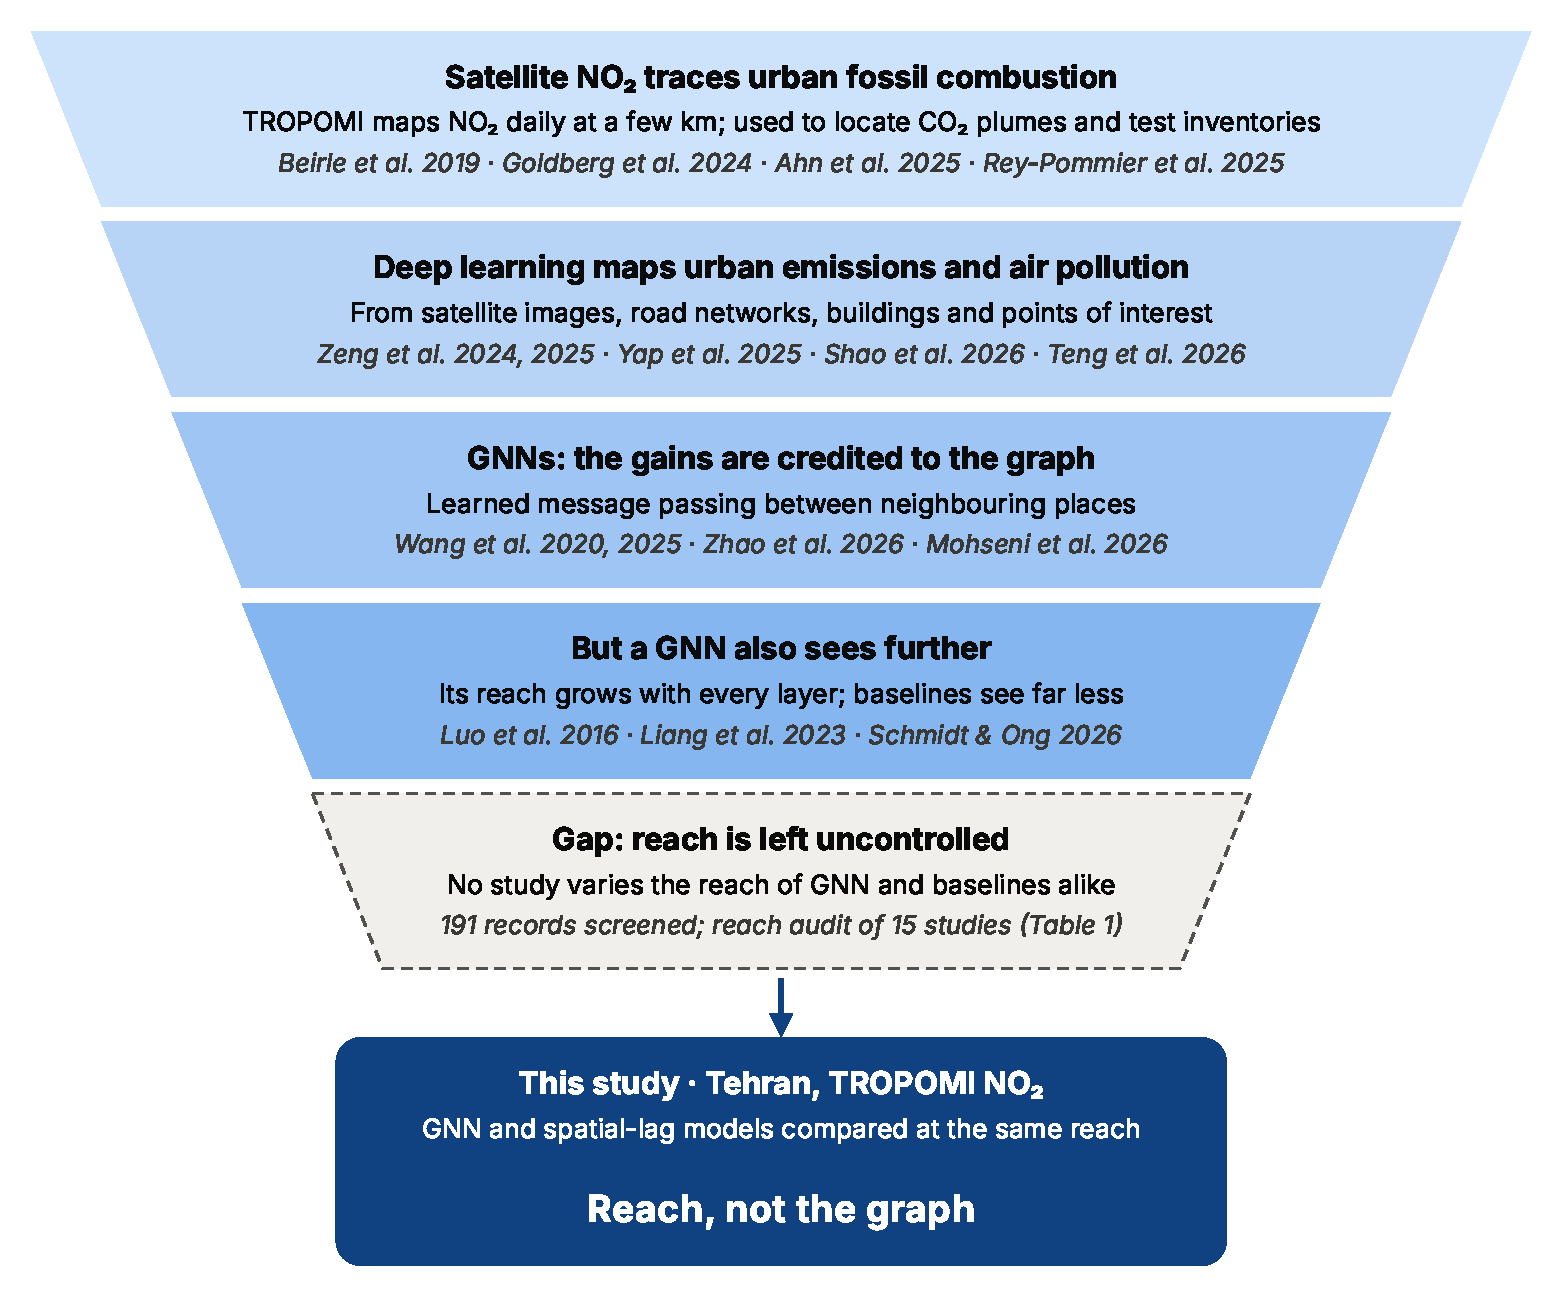
\includegraphics[width=\textwidth]{figures/Fig1.pdf}
\caption{From the literature to the gap. Satellite NO₂ is used as a tracer of urban combustion; deep learning, and graph neural networks in particular, map urban emissions and air pollution, and their gains are credited to the graph. A GNN, however, also sees further than its baselines, and none of the audited studies varied the reach of a GNN and its baselines together under spatial validation}\label{fig:funnel}
\end{figure*}

\section{Study area and data}\label{sec:data}

\subsection{Grid, years and label domain}\label{sec:grid}

The analysis grid covers 50.85--51.90°E and 35.35--35.95°N with 72 × 126 cells of 1/120° (about 0.75 × 0.93 km). The label domain consists of the 2,436 cells of the three central counties (Tehran, Rey and Shemiranat) to which the emission inventory assigns any CO₂. Mountains and desert are thus left out, so a model cannot gain skill simply by telling urban from non-urban cells apart. We use three Iranian (Solar Hijri) years: 1402 (21 March 2023 -- 19 March 2024) and 1403 (20 March 2024 -- 20 March 2025) for development, and 1404 (21 March 2025 -- 20 March 2026) as a held-out year. Fig.~\ref{fig:maps} shows the domain, the observed target of the held-out year and its hotspots.

\begin{figure*}[!htbp]
\centering
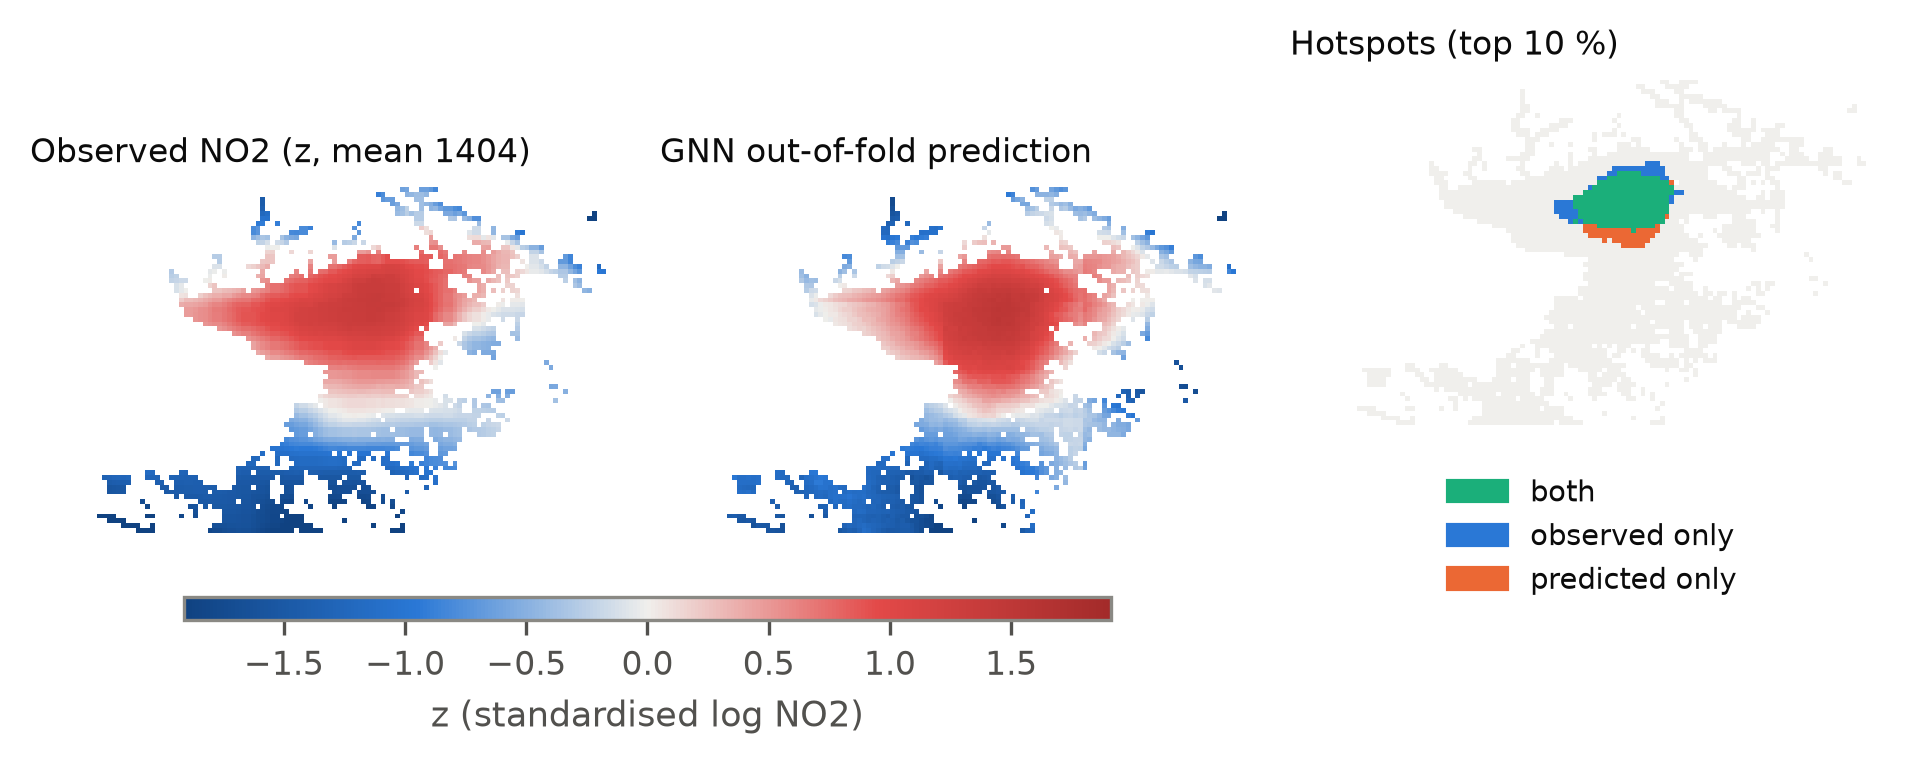
\includegraphics[width=\textwidth]{figures/Fig2.png}
\caption{The label domain and the target in the held-out year 1404. (a) Observed NO₂ pattern: annual mean of the monthly z. (b) Annual mean of the out-of-fold monthly predictions of the five-layer GNN (37.8 km), trained on 1402 and 1403. (c) Hotspots, taken as the top 10\,\% of cells of the two annual mean maps: found by both, by the observation only and by the prediction only. North is up; cells are 1/120° (about 0.84 km)}\label{fig:maps}
\end{figure*}

\subsection{Target}\label{sec:target}

The target is the monthly mean tropospheric NO₂ column of the TROPOMI offline level-3 product in Google Earth Engine (\nolinkurl{COPERNICUS/S5P/OFFL/L3_NO2}, band \nolinkurl{tropospheric_NO2_column_number_density}), which carries the quality filtering that Earth Engine applies when it builds the level-3 product. We drop values below $-0.001$ mol m$^{-2}$, average all remaining scenes of each calendar month on the product's native grid (about 1.1 km), and export the monthly means to the study grid with Earth Engine's default nearest-neighbour resampling. Each Solar Hijri month takes the calendar month with which it overlaps most, and every domain cell has a value in every month. The monthly mean is floored at $10^{-7}$ mol m$^{-2}$ and log-transformed, and the log column is standardised over the domain cells of the month (z), so that only the spatial pattern is kept. A hotspot is a cell whose z is at or above the 90th percentile of its month. Both the standardisation and the threshold use all domain cells of the month and so define the target as a city-wide ranking. They leave the rank metrics of Section~\ref{sec:metrics} unchanged, but they also set the scale of the training targets in every fold. The target is deliberately not the inventory, since a modelled CO₂ map would let a model reproduce the inventory's own allocation.

The target is an extremely smooth field. Its monthly correlogram is 0.95 at 0--2 km and 0.76 at 8--10 km, and it crosses zero at 24 km (Fig.~\ref{fig:correlogram}). The effective number of independent cells \citep{griffith2005} is 4.9 in both development years, against 2,436 cells and about 88 TROPOMI nadir pixels (3.5 × 5.5 km). We compute it as $n^2 / \sum_{i,j} \rho(d_{ij})$ over all pairs of the $n$ cells, with $\rho$ the correlogram pooled over the months of a year (Euclidean distances in 2-km bins, 200,000 random cell pairs), set to zero from the first bin that is not more than two standard errors above zero. It describes the target field, not the number of independent units available to compare two models (Section~\ref{sec:inference}). The pattern is also stable between years. The Spearman correlation between the annual mean maps of any two years is 0.993--0.997, and between the same months it is 0.955--0.963 on average. The main target applies no cloud filter of its own. A target built instead from daily scenes with a cloud fraction below 0.3 agrees with it (Spearman 0.98--0.99; overlap of hotspot sets 0.73--0.76).

The north of the city lies about 700 m higher than the south, and a TROPOMI emission inversion reported terrain artefacts near Mount Tochal \citep{reypommier2025}. Elevation, taken from SRTM and used only for this check, correlates with z ($|\rho| = 0.49$), but partialling it out barely changes model skill (Spearman 0.949 to 0.940). The satellite pattern agrees only weakly with the ranking of the 16--17 stations with NO₂ records inside the grid (mean monthly Spearman 0.11 in 1402 and 0.30 in 1403). It therefore describes column NO₂ rather than street-level concentrations \citep[cf.][]{kafi2026}.

\begin{figure}[!htbp]
\centering
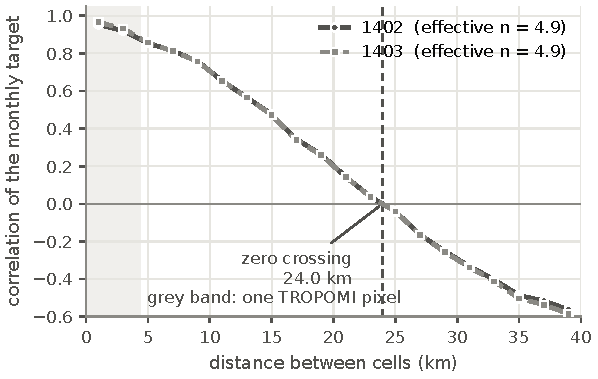
\includegraphics[width=\smallfigwidth]{figures/Fig3.pdf}
\caption{Correlogram of the monthly target in 1402 and 1403 (2-km distance bins). The curve crosses zero at 24.0 km, and the effective number of independent cells is 4.9 of 2,436. Grey band: one TROPOMI pixel (3.5 × 5.5 km)}\label{fig:correlogram}
\end{figure}

\subsection{Predictors}\label{sec:predictors}

The predictors fall into four groups (Table~\ref{tab:predictors}). The traffic and energy layers are estimates, not measurements. The emission layers come from a bottom-up inventory that allocates sector totals to the grid, and the traffic variables come from a traffic assignment model; neither has been checked against measured emissions or traffic counts at the scale of the grid. Monthly sector layers are the annual allocation multiplied by monthly sector shares. No inventory is available yet for 1404, so all models use the 1403 inventory and traffic layers.

\begin{table}[!htbp]
\caption{Predictor groups. The traffic and energy layers are model estimates, not measurements. Years and processing of every layer are described in Table S2 (Online Resource 1)}\label{tab:predictors}
\footnotesize
\begin{tabularx}{\linewidth}{@{}L{1.6cm}Y{1}@{}}
\toprule
Group & Layers \\
\midrule
Traffic & Road-transport CO₂ of a bottom-up inventory (IPCC Tier 1 with Monte Carlo uncertainty, allocated to 1 km); road length by class; peak-hour vehicle-kilometres and volume-to-capacity ratio of a traffic assignment \\
Energy & Residential, commercial, industrial and power-sector CO₂ of the same inventory; monthly heating degree-days \\
Pollution & CO from the 28 stations of the municipal monitoring network, interpolated by inverse distance (power 2) \\
Context & GHSL population, total and non-residential building volume, VIIRS night lights, industrial land share, monthly ERA5-Land temperature and wind speed \\
\botrule
\end{tabularx}
\footnotetext{$\log(1 + x)$ is applied to the inventory CO₂ layers, peak-hour vehicle-kilometres, population, both building volumes and night lights. IPCC, Intergovernmental Panel on Climate Change; GHSL, Global Human Settlement Layer; VIIRS, Visible Infrared Imaging Radiometer Suite; ERA5-Land, land component of the fifth-generation reanalysis of the European Centre for Medium-Range Weather Forecasts}
\end{table}

\section{Methods}\label{sec:methods}

\subsection{Models}\label{sec:models}

All models use the same target and, unless stated otherwise, the same predictors (Table~\ref{tab:predictors}). Table~\ref{tab:models} lists the model families, and Fig.~\ref{fig:design} shows the shared network and how the comparison separates the graph from the reach.

\begin{table}[!htbp]
\caption{Models compared}\label{tab:models}
\footnotesize
\begin{tabularx}{\linewidth}{@{}L{2.2cm}Y{1}@{}}
\toprule
Model & Description \\
\midrule
Own-cell models & Ordinary least squares (OLS), histogram gradient boosting (GBM) and random forests (RF) on the predictors of the cell itself \\
SLX models & The same estimators plus box means of every spatially varying predictor over nested square windows of half-width up to 1, 3, 9, 15, 18, 27, 36 or 45 cells. This is the SLX specification of spatial econometrics and the buffer design of land-use regression. The windows of the original study went up to 15 cells \\
No-graph network & One encoder per input group, a softmax gate over the groups (gated fusion) and a linear head. It is given either no neighbourhood information or the same box means as the SLX models \\
Multi-scale GraphSAGE (GNN) & The same gated encoder followed by $L$ residual GraphSAGE layers \citep{hamilton2017} with mean aggregation over three edge sets: the 8 neighbours at distances of 1, 3 and 9 cells. One layer reaches 9 cells; $L$ layers reach $9L$ cells \\
Physical operator & Gaussian-smoothed inventory layers with one non-negative NO₂ yield per sector; width and yields fitted on the training cells \\
\botrule
\end{tabularx}
\end{table}

For a predictor $x$ (log-transformed where stated in Table~\ref{tab:predictors}) and a cell $i$, the box mean over a half-width of $k$ cells is
\begin{equation}
\bar{x}_i^{(k)} = \frac{1}{(2k+1)^2} \sum_{j:\ \lVert j - i \rVert_\infty \le k} x_j , \label{eq:box}
\end{equation}
that is, the mean over the $(2k+1) \times (2k+1)$ cells centred on $i$, with edge values repeated beyond the grid. SLX models use $x_i$ and $\bar{x}_i^{(k)}$ for every window $k$ of the model, and the no-graph network receives the same box means as extra inputs of each group. In the networks, each input group $m$ (traffic, energy, pollution, context) is encoded to $e_{i,m} = f_m(x_{i,m}) \in \mathbb{R}^{32}$, and a gate weights the groups for every cell and month:
\begin{equation}
\begin{gathered}
a_i = \operatorname{softmax}\!\big(W_g\,[e_{i,1}; \dots ; e_{i,M}] + b_g\big), \\
h_i^{(0)} = \sum_{m=1}^{M} a_{i,m}\, e_{i,m},
\end{gathered} \label{eq:gate}
\end{equation}
with $\sum_m a_{i,m} = 1$. Without a graph, the prediction is $\hat{z}_i = w^{\top} h_i^{(0)} + c$. The GNN applies $L$ residual layers before the same linear head,
\begin{equation}
\begin{split}
h_i^{(l+1)} &= h_i^{(l)} + \operatorname{Dropout}\Big(\operatorname{SiLU}\Big(\sum_{s \in \{1,3,9\}} \big[\, W_s^{(l)} h_i^{(l)} \\
&\qquad + U_s^{(l)} \tfrac{1}{|\mathcal{N}_s(i)|} \sum_{j \in \mathcal{N}_s(i)} h_j^{(l)} \\
&\qquad + b_s^{(l)} \big]\Big)\Big),
\end{split} \label{eq:gnn}
\end{equation}
where $\mathcal{N}_s(i)$ holds the up to 8 cells at offsets $(\pm s, 0)$, $(0, \pm s)$ and $(\pm s, \pm s)$ from $i$, and $\hat{z}_i = w^{\top} h_i^{(L)} + c$. All networks minimise the squared error between $\hat{z}_i$ and the target $z_i$ on the training cells. The two operators differ in how they aggregate neighbourhood information. Eq.~(\ref{eq:box}) averages the inputs over every cell of a window with fixed, equal weights, before the encoders. Eq.~(\ref{eq:gnn}) combines learned representations of sparse stencils, after them.

The edges of the GNN join cells at fixed grid distances and carry no information beyond distance, so the network is close to a dilated convolution with learned, nonlinear aggregation. The comparison therefore tests learned against fixed aggregation up to the same distance. It does not test graphs whose edges carry other information, such as road links, observed travel flows or wind. The decisive control, added after the first results (Section~\ref{sec:prereg}), is the no-graph network fed box means. It shares the GNN's encoder, training, seeds and ensembling, and supplies spatial context as fixed box means instead of learned message passing. The box means use every cell of a square, while the graph uses sparse stencils. The two approaches also differ in how they weight cells and in whether they aggregate before or after the nonlinear encoder. The comparison thus tests two ways of supplying the same maximum reach, rather than one component of the GNN in isolation.

\begin{figure*}[!htbp]
\centering
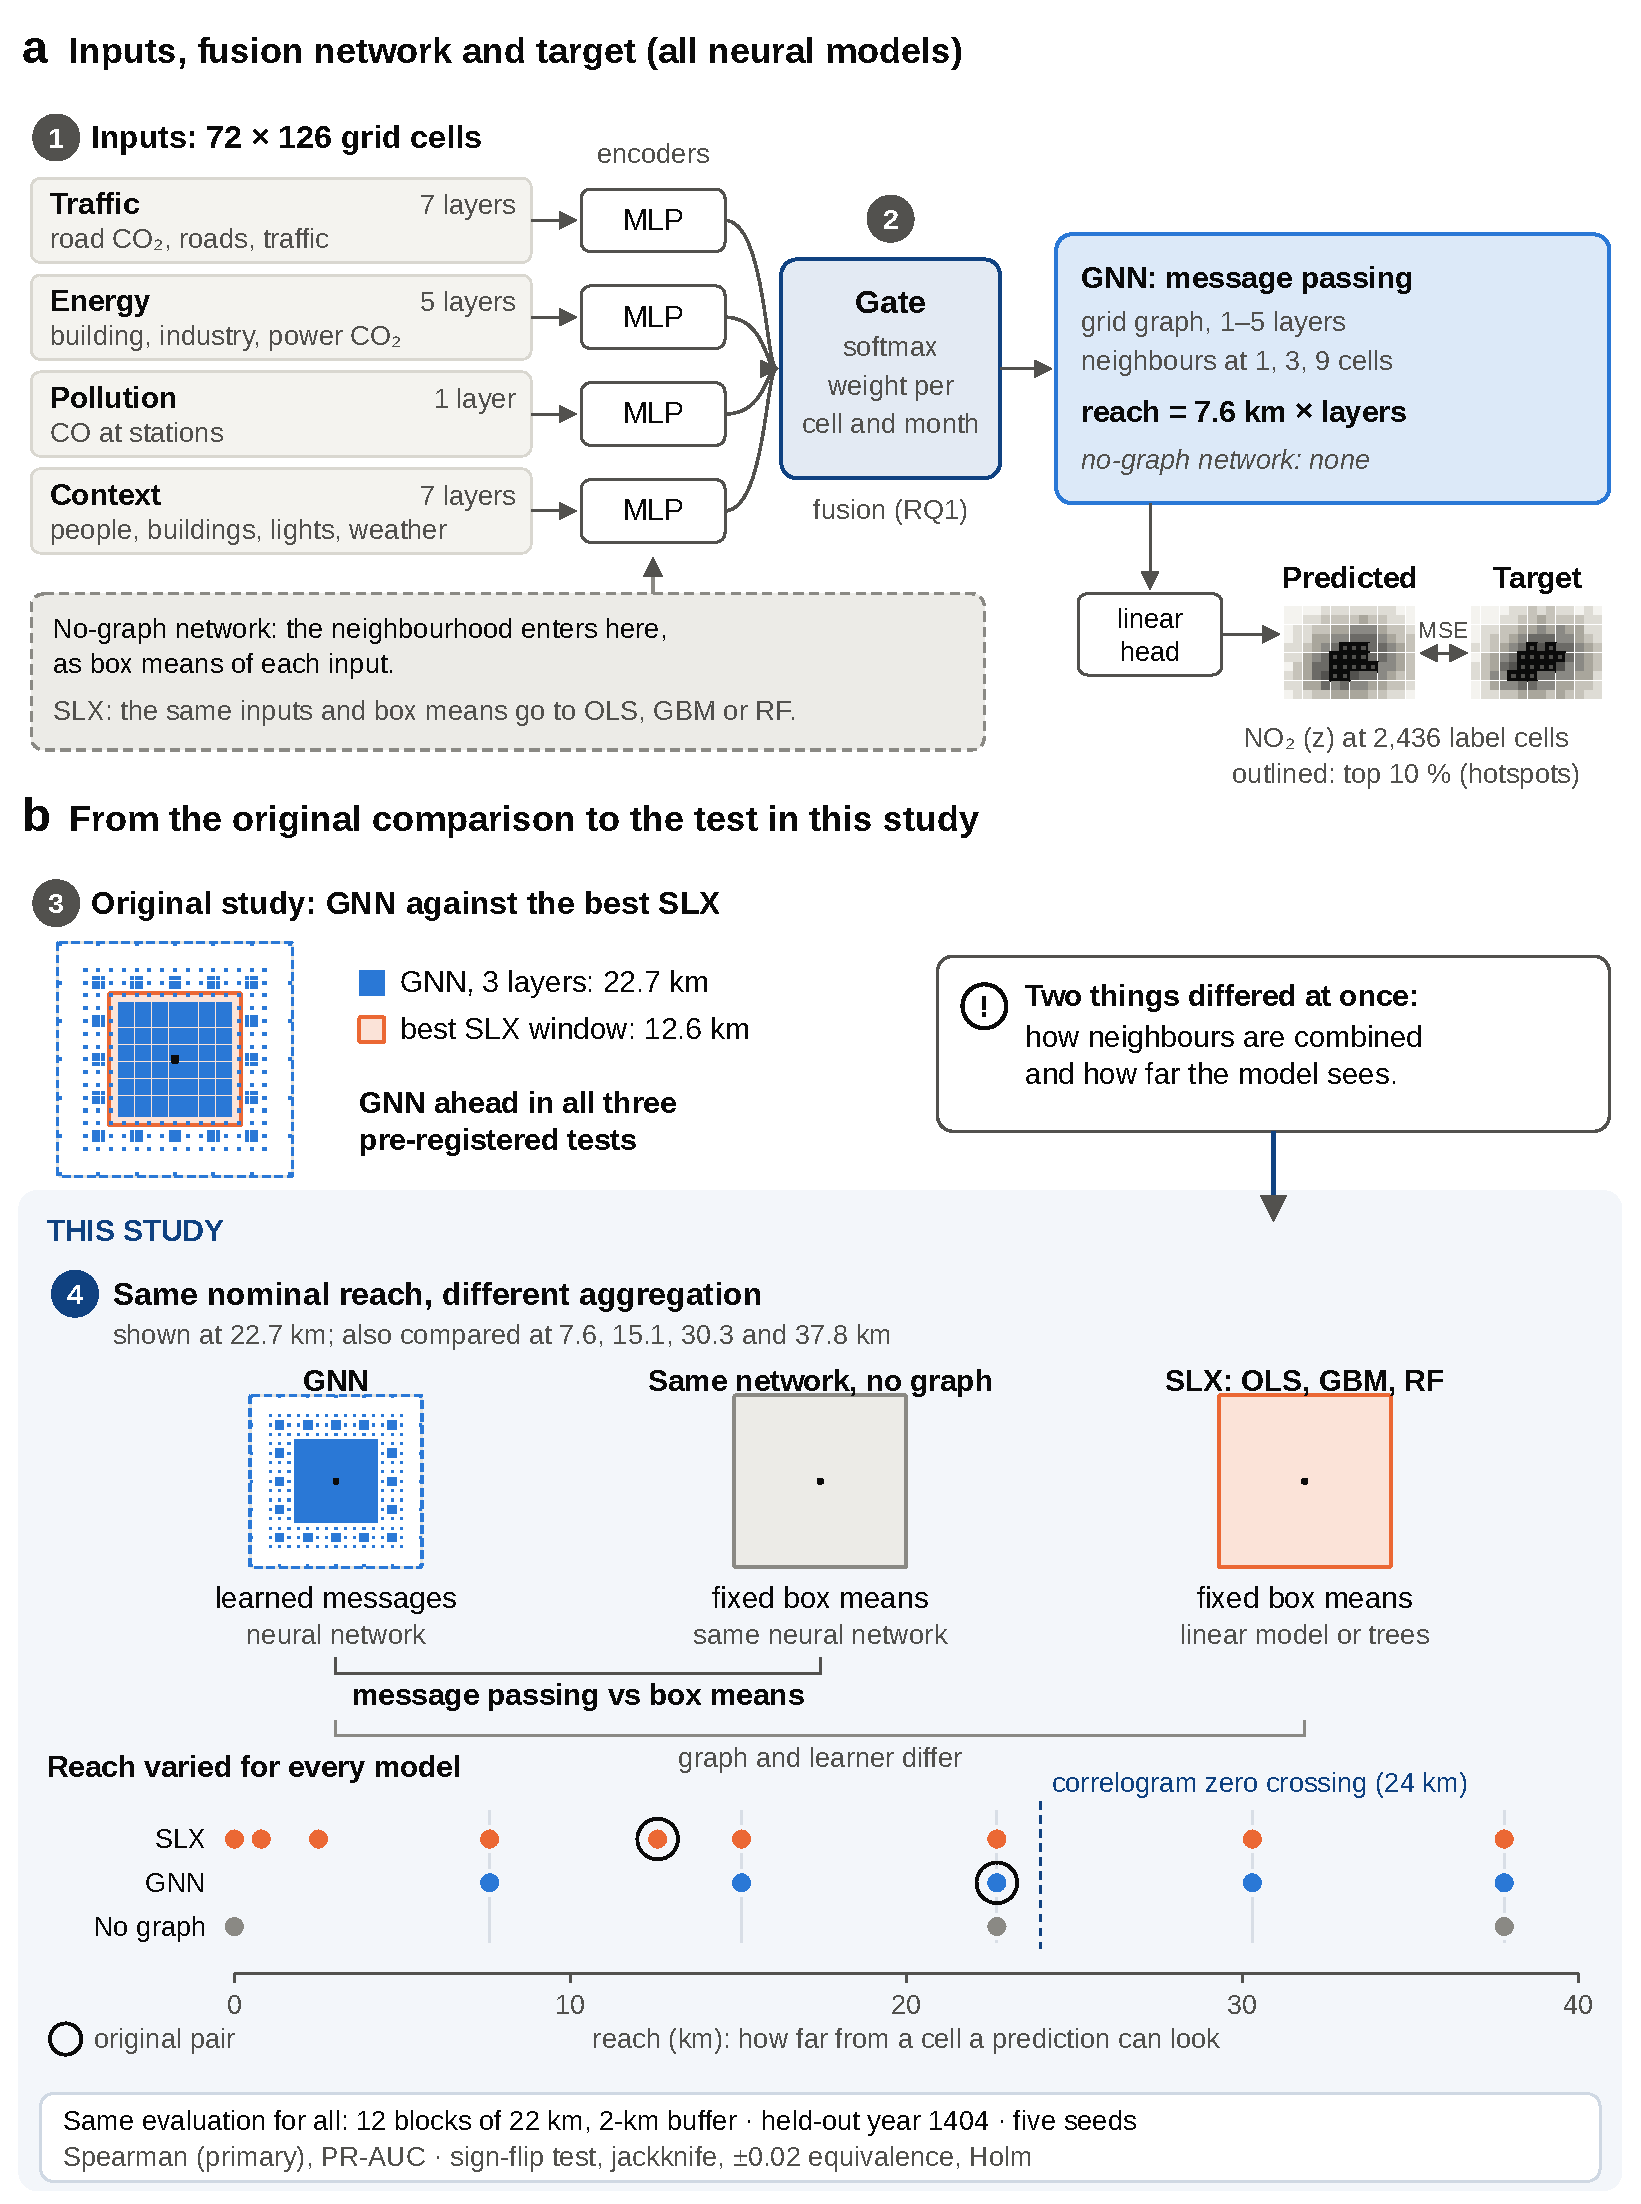
\includegraphics[width=\textwidth,height=0.78\textheight,keepaspectratio]{figures/Fig4.pdf}
\caption{Study design. (a) The network shared by all neural models: one two-layer encoder per input group, a softmax gate that weights the groups for every cell and month (the fusion of RQ1), graph message passing in the GNN only, and a linear head trained on the monthly TROPOMI target (z) with a squared-error loss; hotspots are the top 10\,\% of cells. In the no-graph network the neighbourhood enters instead as box means of each input, and SLX models feed the same inputs and box means to OLS, GBM or RF. (b) The thesis compared a three-layer GNN that sees 22.7 km with SLX models that see at most 12.6 km, so the graph and the reach differed at once. This study compares the GNN with the same network without a graph and with SLX models at the same reach, varies the reach of every family (dots; circles mark the thesis pair), and evaluates all models in the same way. Squares show which cells inform the prediction of the centre cell (black): the sparse stencil of the graph against full box windows. The maps in (a) are schematic}\label{fig:design}
\end{figure*}

Message passing and SLX windows both use the predictors of every grid cell, including those of the held-out block; only the target of held-out cells is unseen. This is the mapping task, in which predictors are known everywhere. All hyper-parameters were fixed before the runs of the original study, and none was tuned here. The neural models use a hidden size of 32, two encoder layers, a dropout of 0.1, AdamW, a learning rate of $3 \times 10^{-3}$ and 300 epochs without early stopping. Every neural model is trained with five seeds. As in the original study, the five predictions are averaged to form a five-seed ensemble, and each individual fit is also scored on its own. OLS is deterministic, and GBM and RF are run with one seed. The fusion networks of RQ1 (Section~\ref{sec:fusion}) are no-graph networks with box means at half-widths of 3 and 9 cells (a reach of 7.6 km).

\subsection{Reach and reach-matched comparisons}\label{sec:reach}

The reach of a model is how far, in cells, a predictor value can be from a cell and still influence its prediction:
\begin{equation}
\begin{gathered}
R = \begin{cases} 9L & \text{GNN, } L \text{ layers (Eq.~\ref{eq:gnn})},\\ \max k & \text{SLX, no-graph network (Eq.~\ref{eq:box})},\\ 0 & \text{own-cell models,} \end{cases} \\
R_{\mathrm{km}} = 0.84\,R ,
\end{gathered} \label{eq:reach}
\end{equation}
Reach is counted in cells on the same grid for every model. Both box windows and graph stencils are square, so reach is a Chebyshev distance. A box window covers every cell within its reach, whereas the graph reaches the same distance through sparse stencils composed over layers and so does not draw on every cell inside the square. Distances in kilometres are nominal and use the mean cell size (0.84 km). Because reach is a Chebyshev distance, a square window reaches farther along its diagonals: the 27-cell window of 22.7 km extends to about 32 km at its corners. Reach is the largest distance a model can use; its effective receptive field may be shorter \citep{luo2016}. We call a comparison reach-matched when the models have the same reach in cells. The GNN was run with one to five layers (7.6--37.8 km) in cross-validation and with four and five layers on the held-out year. SLX models were run at 0--37.8 km, and the no-graph network at 0, 22.7 and 37.8 km.

As a heuristic for the reach a task needs, we use the distance $R^{*}$ at which the correlogram of the target first crosses zero (24.0 km; Section~\ref{sec:target}). In nominal terms this is close to the 27-cell (22.7 km) reach of a three-layer GNN, but the correlogram uses Euclidean distances, so the two numbers measure distance differently. $R^{*}$ is not a physical constant, though. The target is standardised over a bounded domain and has a large-scale gradient, and its zero crossing depends on both. It falls to 19.3--19.4 km after a planar trend is removed and to 13.9--14.1 km after a quadratic trend is removed, and to 21.5--21.7 km and 18.0--18.3 km on domains cropped to 80\,\% and 60\,\% of their extent. $R^{*}$ was computed after the first runs, so results near it are consistent with the heuristic but do not test it blindly.

\subsection{Validation}\label{sec:validation}

The domain is divided into 22-km square blocks (the autocorrelation range estimated for the original design), which gives 12 blocks. Each block is held out once, and training cells within 2 km of it are removed. In cross-validation, models are trained and tested within each development year (1402 or 1403) separately. For the held-out year, each fold trains on the training blocks of 1402 and 1403 and predicts the held-out block in 1404. This tests prediction at new locations in a new year \citep{meyer2018}. The target changes little between years (Section~\ref{sec:target}), so the held-out year mainly tests stability and provides little new information.

The station layer was originally interpolated once from all stations, including those inside the test block. Here it is rebuilt for every fold from the stations farther than 2 km from the test block, which in one fold removes 19 of the 28 stations. The 2-km buffer is short compared with the correlation length, so cross-validation measures interpolation within the city more than extrapolation. We therefore also ran the reach-matched comparison with buffers of 10 and 20 km. With a 20-km buffer, no station remains in 4 of the 12 folds, so these runs use only the driver inputs (traffic, energy and context), and the 2-km runs were repeated with the same inputs for comparison.

\subsection{Metrics}\label{sec:metrics}

The primary metric is the Spearman correlation between predicted and observed z over the domain cells, averaged over months. We also report the area under the precision--recall curve of the hotspot label (PR-AUC), computed as average precision for each month over the domain cells and averaged over months like the Spearman correlation. Its chance level is the hotspot share (0.10). It is a descriptive measure only: the hotspots of a month form a few contiguous areas, so PR-AUC rests on very few independent units. Sensitivity analyses use hotspot labels at the top 20\,\% and top 5\,\% (chance levels 0.20 and 0.05), and the same metrics on superpixels of 5 × 5 cells, about one TROPOMI pixel. To measure how much of the skill is due to the smoothness of the target alone, we also interpolate the target of the training cells of the same month, with the same folds and buffer, by inverse-distance weighting and by a Gaussian process on the coordinates. These baselines use the target of the same month and are therefore interpolation, not prediction from predictors.

\subsection{Inference with few spatial blocks}\label{sec:inference}

Differences between two models are computed from their out-of-fold predictions for the same cells and months. The main test is a block sign-flip randomisation test that enumerates all $2^{12} = 4{,}096$ assignments. After the predictions are rank-normalised within each month, the predictions of the two models are swapped block by block, with the same swap in every month, and the city-wide difference of the metric is recomputed. Enumeration makes the test exhaustive, but its validity rests on the blocks being exchangeable under the null hypothesis, which dependence between neighbouring blocks only approximates (see below). All 12 blocks enter this test, also for PR-AUC, because blocks without hotspots still contribute negative cells. As a check, the test is also applied to the cell-weighted mean of per-block differences.

Intervals are delete-one-block jackknife intervals with $K - 1$ degrees of freedom: each block is removed in turn, and the city-wide difference is recomputed from the other eleven. With $\Delta = M_{\mathrm{cand}} - M_{\mathrm{ref}}$ the difference of a metric $M$ (averaged over months) and $\Delta_{(-b)}$ the same difference without block $b$,
\begin{equation}
\begin{gathered}
\widehat{\mathrm{SE}} = \sqrt{\frac{K-1}{K} \sum_{b=1}^{K} \big(\Delta_{(-b)} - \bar{\Delta}_{(\cdot)}\big)^2}, \\
\mathrm{CI}_{1-\alpha} = \Delta \pm t_{1-\alpha/2,\,K-1}\, \widehat{\mathrm{SE}}, 
\end{gathered} \label{eq:jackknife}
\end{equation}
with $K = 12$ blocks and $\bar{\Delta}_{(\cdot)}$ the mean of the $K$ leave-one-out differences.

Each comparison receives one of five verdicts, applied in this order \citep[two one-sided tests for equivalence;][]{lakens2017}, with $[\ell_{95}, u_{95}]$ and $[\ell_{90}, u_{90}]$ the intervals of Eq.~(\ref{eq:jackknife}) and margin $\delta$:
\begin{equation}
\text{verdict} = \begin{cases} \text{superior} & \ell_{95} > 0,\\ \text{equivalent} & -\delta < \ell_{90} \text{ and } u_{90} < \delta,\\ \text{non-inferior} & \ell_{95} > -\delta,\\ \text{inferior} & u_{95} < 0,\\ \text{inconclusive} & \text{otherwise.} \end{cases} \label{eq:verdict}
\end{equation}
Superiority is checked first, so a difference whose 95\,\% interval lies entirely above zero is called superior even if it is smaller than the margin. Equivalence is checked before inferiority, so a difference whose 95\,\% interval lies entirely below zero but whose 90\,\% interval lies inside $\pm\delta$ is called equivalent: it is detectable but smaller than the margin. The registration set $\delta = 0.02$ for Spearman, the larger of 0.02 and twice the seed-to-seed standard deviation measured then (0.0077). This margin is about a tenth of the gain from no neighbourhood to a reach of 12.6 km. PR-AUC verdicts use the same margin but are descriptive. The verdicts come from the unadjusted intervals. These intervals are nominal and conditional on the fitted predictions: they do not include the variation from retraining the models. The randomisation tests are one-sided, in the direction of the candidate (usually the GNN) being better. Holm's adjustment \citep{holm1979} is applied to the randomisation p-values within each family: the 22 primary comparisons of the registered family, and separately the exploratory comparisons of this study. Table S1 (Online Resource 1) lists every comparison with both interval levels, unadjusted and adjusted p-values and family. The block bootstrap of the original study is reported for comparison.

The correlation length (24 km) exceeds the block size, so neighbouring blocks are dependent and the nominal level of the randomisation test is only approximate. As a diagnostic, we applied the test to 20 comparisons between pairs of individual fits of the same GNN (five seeds, two years), which have no true difference in expectation. The pairs share data and seeds, so this checks calibration only roughly. For PR-AUC, 1 of the 20 comparisons fell below $p = 0.05$, as expected; for Spearman, 5 of 20 did. The test is therefore liberal for Spearman, and we read significant Spearman p-values with caution. A liberal test does not make non-significant results more precise, since the precision of each comparison is given by its interval. Finally, the effective number of independent cells of the target (Section~\ref{sec:target}) describes the target field. It indicates, but does not equal, the information available to compare two models.

\subsection{Pre-registration, transparency and use of AI tools}\label{sec:prereg}

This paper re-examines the model comparison of an unpublished master's thesis by one of the authors, the ``original study'', whose models, windows, folds and hyper-parameters are reused unless stated otherwise. Its decision rules, including a held-out-year test on 1404, were written before any model was evaluated. The checks of this paper (reach-matched SLX models, the leakage control, the physical operator and the inference rules) were registered before the corresponding runs. The registrations are timestamped by the project's version control, and deviations are listed in the registration documents. A planned second held-out year (1405) and a hyper-parameter search were registered but not carried out. The GNN depth curve, the no-graph network with box means, the short SLX windows, the larger buffers and the interpolation baselines were added after the first results and are exploratory. All runs used one RTX 4080 GPU, and every run is logged with its configuration hash, data hash and code version.

The authors used Claude (Anthropic), a large language model, to help write and review the analysis code and to draft and edit parts of the text. The analysis code is checked by automated tests, and every reported number comes from a logged run with its configuration and code version. The authors reviewed and edited the content as needed and take full responsibility for the content of the article.

\section{Results}\label{sec:results}

\subsection{Skill rises with reach and levels off}\label{sec:curve}

SLX models and the GNN improve steeply as they are allowed to see further, and then gain much less (Fig.~\ref{fig:reach}, Table~\ref{tab:reach}). Models restricted to their own cell reach a Spearman correlation of 0.66--0.77. SLX models gain little from the nearest cells (0.73--0.79 at 0.8--2.5 km), but reach 0.86--0.87 at 7.6 km and 0.91--0.93 at 12.6 km. Beyond that they gain less: at 22.7--37.8 km they reach 0.92--0.95, and the best SLX model gains a further 0.026 in 1402 and 0.003 in 1403 from 12.6 to 37.8 km. The GNN follows the same curve, from 0.90--0.91 with one layer (7.6 km) to 0.94 with two layers and 0.95 with three to five, with no gain beyond three layers. The no-graph network scores 0.68 without neighbourhood information and 0.954--0.958 with box means extending to 22.7 or 37.8 km. It was run at these three reaches only, so its curve between them is not known. Gains thus become small beyond 12--23 km. This range overlaps the correlation length after the large-scale trend is removed (14--19 km; Section~\ref{sec:reach}) and lies below the raw zero crossing (24 km). PR-AUC follows the same pattern, with more scatter between estimators and years.

\begin{table*}[!htbp]
\caption{Cross-validated Spearman correlation against reach, 1402 / 1403. SLX: the best of OLS, GBM and RF at each reach (estimator in brackets; Fig.~\ref{fig:reach} shows every estimator). Networks: five-seed ensembles}\label{tab:reach}
\footnotesize
\begin{tabular}{@{}llll@{}}
\toprule
Reach (km) & Best SLX & GNN & No-graph network \\
\midrule
0 & 0.768 (GBM) / 0.745 (GBM) & -- & 0.685 / 0.676 \\
0.8 & 0.767 (GBM) / 0.757 (GBM) & -- & -- \\
2.5 & 0.780 (GBM) / 0.788 (GBM) & -- & -- \\
7.6 & 0.866 (RF) / 0.868 (OLS) & 0.902 / 0.907 & -- \\
12.6 & 0.924 (GBM) / 0.934 (OLS) & -- & -- \\
15.1 & 0.921 (GBM) / 0.924 (OLS) & 0.938 / 0.942 & -- \\
22.7 & 0.938 (OLS) / 0.934 (GBM) & 0.949 / 0.947 & 0.954 / 0.955 \\
30.3 & 0.942 (OLS) / 0.933 (GBM) & 0.950 / 0.949 & -- \\
37.8 & 0.950 (GBM) / 0.937 (RF) & 0.946 / 0.946 & 0.958 / 0.956 \\
\botrule
\end{tabular}
\end{table*}

\begin{figure*}[!htbp]
\centering
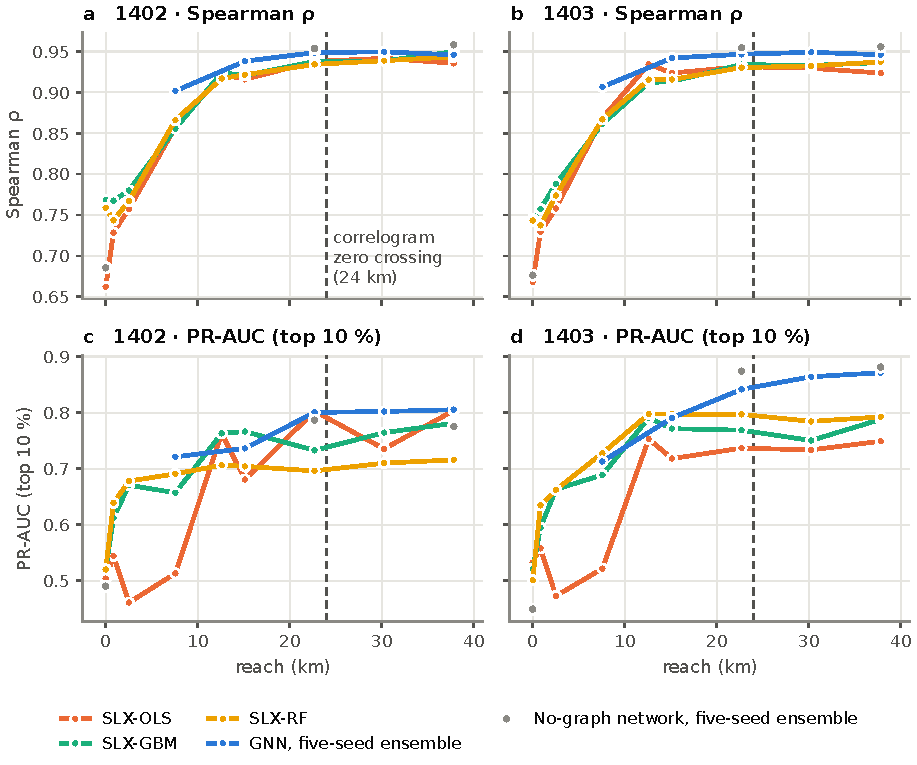
\includegraphics[width=\textwidth]{figures/Fig5.pdf}
\caption{Skill against reach under 22-km block cross-validation, Spearman (a, b) and PR-AUC (c, d), 1402 (left) and 1403 (right). Lines: SLX models and the GNN with growing reach (five-seed ensembles for the GNN). Points: the no-graph network, run at 0, 22.7 and 37.8 km. Dashed line: zero crossing of the target correlogram (24 km)}\label{fig:reach}
\end{figure*}

\subsection{At equal reach, the graph adds little over neighbourhood means}\label{sec:equal}

Table~\ref{tab:equal} compares the GNN at each depth with models of exactly the same reach. Against SLX models, the GNN's lead in Spearman shrinks as reach grows: about 0.04 at 7.6 km, 0.02 at 15.1 km, 0.011--0.016 at 22.7--30.3 km, and −0.004 and +0.009 at 37.8 km. None of these differences is significant after Holm adjustment, and all jackknife intervals include zero. For individual fits the leads are smaller still (0.028--0.033 at 7.6 km, 0.007--0.008 at 22.7 km, −0.008 and +0.005 at 37.8 km). Part of the GNN's lead over SLX at short reach therefore comes from its learner and ensemble, and the lead disappears where skill levels off. In PR-AUC, the GNN ensemble leads the SLX references by 0.02--0.11 at 22.7--37.8 km, and several jackknife intervals exclude zero. No randomisation test is significant after Holm adjustment, though, and the single-seed leads are about half as large (0.035--0.073 at 22.7 km, −0.007 to +0.055 at 37.8 km).

The no-graph network fed box means, an exploratory control (Section~\ref{sec:prereg}), shares the GNN's encoder, training, seeds and ensemble, and differs in how spatial context is supplied (Section~\ref{sec:models}). At 22.7 km it is statistically equivalent to the GNN in both years, and slightly better (Spearman −0.005 and −0.008 for GNN minus no-graph network, 90\,\% intervals inside ±0.02). At 37.8 km it is again slightly better (−0.012 and −0.010): equivalent in 1403 and inconclusive in 1402. In 1403 the nominal 95\,\% intervals exclude zero at both reaches, so the box-mean network is detectably, though not materially, better. In PR-AUC the difference changes sign between years at both reaches (+0.014 and −0.032 at 22.7 km; +0.030 and −0.010 at 37.8 km). For the ranking, then, replacing message passing by fixed neighbourhood means cost nothing at these reaches; for the hotspots, the evidence favours neither.

\begin{table*}[!htbp]
\caption{GNN (five-seed ensemble) minus a reference of equal reach, Spearman, cross-validation, 1402 / 1403. SLX: at each reach, the estimator with the best mean Spearman over 1402 and 1403 (RF at 7.6 km, OLS at 15.1 km, GBM at 22.7--37.8 km), so the differences can differ from those implied by the per-year best in Table~\ref{tab:reach}. Intervals: delete-one-block jackknife, 95\,\%. $p$: one-sided block sign-flip test over all 4,096 assignments, unadjusted (liberal for Spearman; Section~\ref{sec:inference}). None is significant after Holm adjustment within the exploratory family}\label{tab:equal}
\footnotesize
\setlength{\tabcolsep}{4.5pt}
\begin{tabular}{@{}lL{2.1cm}lllll@{}}
\toprule
Reach & Reference & \st{$\Delta$ 1402}{[95\,\% CI]} & $p$ & \st{$\Delta$ 1403}{[95\,\% CI]} & $p$ & Verdict \\
\midrule
7.6 km & SLX & \st{+0.036}{[−0.024, +0.096]} & 0.033 & \st{+0.040}{[−0.020, +0.100]} & 0.027 & inconclusive \\
15.1 km & SLX & \st{+0.022}{[−0.041, +0.085]} & 0.15 & \st{+0.018}{[−0.035, +0.072]} & 0.17 & inconclusive \\
22.7 km & SLX & \st{+0.011}{[−0.034, +0.056]} & 0.11 & \st{+0.013}{[−0.028, +0.053]} & 0.056 & inconclusive \\
30.3 km & SLX & \st{+0.011}{[−0.023, +0.046]} & 0.084 & \st{+0.016}{[−0.026, +0.059]} & 0.042 & inconclusive \\
37.8 km & SLX & \st{−0.004}{[−0.035, +0.028]} & 0.79 & \st{+0.009}{[−0.031, +0.050]} & 0.14 & inconclusive \\
22.7 km & No-graph network, box means & \st{−0.005}{[−0.017, +0.007]} & 0.93 & \st{−0.008}{[−0.016, −0.001]} & 0.92 & equivalent \\
37.8 km & No-graph network, box means & \st{−0.012}{[−0.030, +0.005]} & 0.995 & \st{−0.010}{[−0.017, −0.003]} & 0.98 & \st{inconclusive /}{equivalent} \\
\botrule
\end{tabular}
\end{table*}

The comparison in the original study came out differently because its reference models had a shorter reach. Against SLX-GBM at 12.6 km, the pre-specified reference, the three-layer GNN led by +0.025 and +0.035 in Spearman (randomisation $p = 0.001$ and 0.0007; Holm-adjusted 0.021 and 0.016) and by +0.037 and +0.051 in PR-AUC. These leads are partly a comparison of reaches. Given the liberal behaviour of the Spearman test, even the remaining part is uncertain: the jackknife intervals include zero (−0.003 to +0.052 and −0.013 to +0.082), and the block-level version of the test is not significant ($p = 0.058$ and 0.055). Fig.~\ref{fig:diff} shows the differences against the pre-specified and against extended-reach references.

\begin{figure*}[!htbp]
\centering
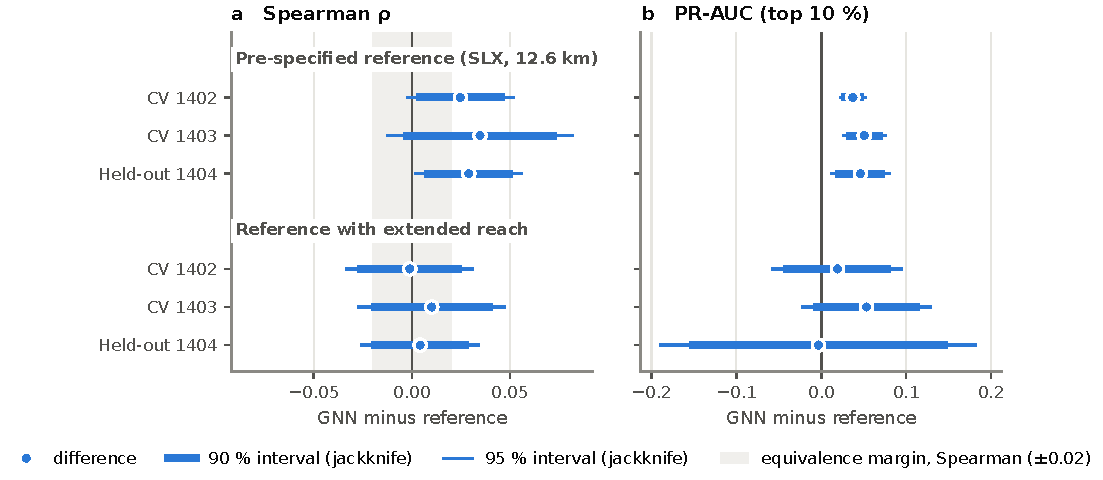
\includegraphics[width=\textwidth]{figures/Fig6.pdf}
\caption{GNN (five-seed ensemble; three layers, 22.7 km, in cross-validation and five layers, 37.8 km, on 1404) minus reference in Spearman (a) and PR-AUC (b), with 90\,\% (thick) and 95\,\% (thin) delete-one-block jackknife intervals. Upper rows: the pre-specified references of the original study (SLX-GBM at 12.6 km in cross-validation, SLX-RF at 12.6 km on the held-out year). Lower rows: references with extended reach (the best SLX model by Spearman at any reach in cross-validation; SLX-OLS at 22.7 km on the held-out year, shorter than the GNN's 37.8 km; the comparisons at exactly equal reach are in Table~\ref{tab:holdout}). Grey band in (a): equivalence margin (±0.02)}\label{fig:diff}
\end{figure*}

\subsection{On the held-out year, GNN and SLX at equal reach have almost the same Spearman correlation}\label{sec:holdout}

In 1404, the five-layer GNN (37.8 km) scores 0.933 in Spearman correlation and 0.782 in PR-AUC, and the four-layer GNN (30.3 km) scores 0.931 and 0.785 (Table~\ref{tab:holdout}). At 30.3 km, the best SLX model (OLS, 0.934) is statistically equivalent to the GNN (−0.003, 95\,\% interval −0.019 to +0.014). At 37.8 km, the best SLX model (RF, 0.932) differs by +0.002 (95\,\% interval −0.026 to +0.029; inconclusive). Here the SLX reference is the estimator with the best Spearman at that reach. In PR-AUC the five-seed ensembles lead this reference by 0.049--0.086, and lead the SLX estimator with the best PR-AUC at each reach by 0.043--0.058. Individual fits lead by less: the mean single seed scores 0.758 at 30.3 km and 0.741 at 37.8 km, against 0.699 and 0.733 for the references. A linear SLX model with a shorter reach of 22.7 km (OLS) does as well as either GNN (0.929 and 0.785), although it was chosen among fifteen variants after the results, which favours it. Its whole held-out-year run (12 folds, trained on 1402 and 1403) took 8 s on one CPU, against 39 min on one RTX 4080 GPU for the five-layer GNN (12 folds, five seeds); both are wall-clock times of the logged runs.

Against the pre-specified reference of the original study (SLX-RF at 12.6 km), the five-layer GNN led in Spearman by +0.029 (95\,\% interval +0.001 to +0.056, $p = 0.0095$). This is not significant after Holm adjustment over the registered family ($p = 0.19$).

\begin{table*}[!htbp]
\caption{Held-out year 1404: GNN and SLX at equal reach, and a shorter-reach SLX model. GNN: five-seed ensemble, and the mean of its individual fits. Differences in the text are computed from unrounded values}\label{tab:holdout}
\footnotesize
\begin{tabular}{@{}lL{4.3cm}ll@{}}
\toprule
Reach & Model & Spearman & PR-AUC \\
\midrule
30.3 km & GNN, 4 layers & 0.931 & 0.785 \\
 & GNN, 4 layers, mean of individual fits & 0.926 & 0.758 \\
 & SLX-OLS / SLX-RF / SLX-GBM & 0.934 / 0.923 / 0.914 & 0.699 / 0.727 / 0.641 \\
37.8 km & GNN, 5 layers & 0.933 & 0.782 \\
 & GNN, 5 layers, mean of individual fits & 0.928 & 0.741 \\
 & SLX-OLS / SLX-RF / SLX-GBM & 0.930 / 0.932 / 0.927 & 0.739 / 0.733 / 0.664 \\
22.7 km & SLX-OLS & 0.929 & 0.785 \\
\botrule
\end{tabular}
\end{table*}

\subsection{Seed averaging hides instability}\label{sec:seeds}

Across seeds, the standard deviation of the GNN's Spearman correlation is about 0.005, but that of its PR-AUC is 0.028 in 1402, 0.038 in 1403 and 0.075 in 1404. In 1403 the individual fits range from 0.756 to 0.858 in PR-AUC (Fig.~\ref{fig:seeds}). Averaging five seeds raises PR-AUC by 0.03--0.04 (for example 0.800 against 0.771 in 1402) and Spearman by about 0.005. The SLX models were run once and so get no such benefit, and a comparison of a five-seed ensemble with single baselines favours the network by about the size of the PR-AUC leads reported in Section~\ref{sec:equal}. This is why the GNN's PR-AUC leads at equal reach (Sections~\ref{sec:equal} and \ref{sec:holdout}) are smaller and more variable for individual fits. Whether ensembling the stochastic SLX baselines would close the gap was not tested.

\begin{figure*}[!htbp]
\centering
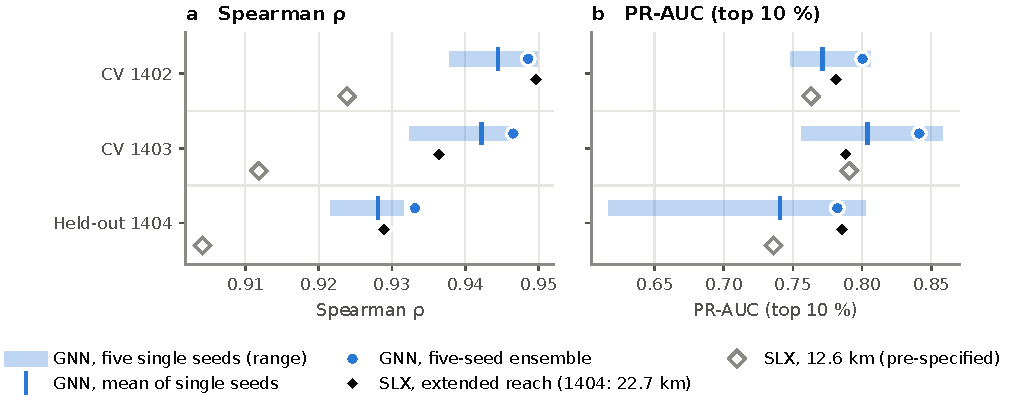
\includegraphics[width=\textwidth]{figures/Fig7.pdf}
\caption{Seeds against ensemble, Spearman (a) and PR-AUC (b), with three lanes per row so that close values stay visible. Upper lane: the GNN, three layers (22.7 km) in cross-validation and five layers (37.8 km) on 1404 (bar: range of the five individual fits; tick: their mean; dot: five-seed ensemble). Middle lane: SLX with extended reach (best SLX model by Spearman at any reach in cross-validation; SLX-OLS at 22.7 km on 1404). Lower lane: the pre-specified SLX reference at 12.6 km}\label{fig:seeds}
\end{figure*}

\subsection{How the evaluation decides the verdict}\label{sec:verdict}

The original study's confirmatory test on 1404 compared the GNN with the pre-specified SLX-RF at 12.6 km in PR-AUC. With the block bootstrap the difference was +0.065 (95\,\% interval +0.013 to +0.163), and the hypothesis was declared supported. Using the same predictions and the procedure of Section~\ref{sec:inference}, the jackknife interval is −0.019 to +0.149 and the randomisation $p$-value is 0.10. The verdict is then non-inferior, because the lower bound is above −0.02. With the leakage-free predictions of this paper, the difference is +0.046 and the jackknife interval (+0.011 to +0.082) calls the GNN superior, but the randomisation $p$ is 0.098, and 1.0 after Holm adjustment. With an effective sample size of about five independent cells in the target, procedures that are each defensible disagree, and the choice of inference decides between ``significantly better'' and ``no evidence of a difference''.

\subsection{Fusion of data sources does not clearly help (RQ1)}\label{sec:fusion}

Under the same gated network, fusing the estimated traffic and energy layers with station data did not consistently beat the best single source (energy, pre-specified in the registration). In PR-AUC the fused model scored +0.022 and +0.040 higher (95\,\% intervals −0.013 to +0.057 and −0.010 to +0.091; non-inferior). In Spearman it scored 0.021 and 0.022 lower, for all five seeds, but with wide intervals (inconclusive). On 1404, where the registered design compares four-layer GNNs, fused and energy-only models were equivalent in Spearman (−0.007, 90\,\% interval −0.019 to +0.005) and differed by −0.011 in PR-AUC (inconclusive). Fusion thus helps neither metric clearly, and the sign of its effect depends on the metric.

Two observations are consistent with this. First, urban form already gives the ranking. A network with urban-form context alone (population, building volume, night lights) reaches a Spearman correlation of 0.91, though only 0.58--0.59 in PR-AUC, and the emission layers sharpen the top of the ranking rather than the ranking itself. Second, the two largest emission layers are redundant at the scale of the target. Estimated road and building CO₂ correlate at 0.58 for single cells but at 0.998--0.999 once smoothed over 8 km or more, the scale over which the target varies. Both are allocations of the same inventory, so part of this redundancy may come from how the inventory distributes sector totals (Section~\ref{sec:limitations}). We checked it only for these two layers. Whether the station layer and the other inputs are equally redundant was not tested, so the shared explanation for fusion and the graph remains a hypothesis: at the scale that matters, different inputs and different ways of combining a neighbourhood carry the same information.

After the station layer was rebuilt without the test-block stations, the station-only network reached a PR-AUC of 0.715 and 0.726, against 0.648 and 0.691 with the original pre-processing. Leakage therefore did not inflate the original results for this model and metric. A physical operator with one NO₂ yield per sector reached a Spearman correlation of 0.85 and a PR-AUC of 0.51--0.55. This is far better than the original operator, which smoothed all sectors together (PR-AUC 0.35), but below every SLX model with a reach of 12.6 km or more. As the operator uses the inventory layers only, this comparison does not isolate physics from learning.

\subsection{What the target allows}\label{sec:target-limits}

Much of the skill comes from the smoothness of the target itself. Interpolating the target of the training cells of the same month, without any environmental predictor, reaches a Spearman correlation of 0.86 and 0.81 (1402 and 1403) with a Gaussian process on the coordinates and 0.68--0.69 with inverse-distance weighting (PR-AUC 0.72 and 0.61, and 0.34--0.37). The predictors and models add about 0.08--0.14 in Spearman to the Gaussian process, and the GNN and the reach-matched SLX models add the same amount.

Under other hotspot definitions and on superpixels, the picture is similar (Table~\ref{tab:sens}). Against the shorter-reach references, the GNN ensemble leads under every definition. Against references with extended reach, SLX models rank better on superpixels in cross-validation (−0.027 and −0.017), while the GNN ensemble leads at the top 20\,\% and 5\,\% in 1403 (+0.040 and +0.116). On superpixels, the target and predictions are averaged within each superpixel (partial superpixels included) and the top-10\,\% label is recomputed. The top-5\,\% label marks about 120 cells per month in a few contiguous areas. These values therefore rest on very few independent units, and single-seed values are not available for them.

\begin{table*}[!htbp]
\caption{GNN (five-seed ensemble) minus reference under other hotspot definitions and on 5 × 5-cell superpixels (delete-one-block jackknife estimates; intervals in Table S1, Online Resource 1)}\label{tab:sens}
\footnotesize
\begin{tabular}{@{}L{3.1cm}lllll@{}}
\toprule
Reference & Year & \st{PR-AUC,}{top 20\,\%} & \st{PR-AUC,}{top 5\,\%} & \st{Spearman,}{superpixels} & \st{PR-AUC,}{superpixels} \\
\midrule
SLX-GBM, 12.6 km & 1402 & +0.025 & +0.044 & +0.026 & +0.026 \\
 & 1403 & +0.027 & +0.144 & +0.041 & +0.024 \\
SLX-RF, 12.6 km & 1404 & +0.025 & +0.049 & +0.033 & +0.022 \\
Best SLX by Spearman, any reach & 1402 & +0.014 & +0.028 & −0.027 & +0.011 \\
 & 1403 & +0.040 & +0.116 & −0.017 & +0.035 \\
SLX-OLS, 22.7 km & 1404 & −0.013 & +0.002 & +0.008 & −0.025 \\
\botrule
\end{tabular}
\end{table*}

Larger buffers, which force the models to extrapolate from the periphery towards the centre, change the picture (driver inputs, reach 22.7 km). With the 2-km buffer used elsewhere in this paper, the GNN and the best SLX model are level (Spearman 0.943 and 0.945 against 0.940 and 0.935). With a 10-km buffer, the GNN keeps 0.913 and 0.911, while the best SLX model falls to 0.856 and 0.845. With a 20-km buffer, the GNN keeps 0.791 and 0.774, while SLX models fail (best 0.35 and 0.24); the model in the central fold then trains on only 270 peripheral cells. Larger buffers thus change both the distance to the training cells and the number of training cells, and the two effects are not separated here. Tree ensembles cannot predict beyond the range of their training targets and OLS extrapolates wildly, so the failure is one of the conventional learners. Whether the GNN's robustness comes from the graph or from the neural learner was not tested, because the no-graph network was not run with larger buffers.

\section{Discussion}\label{sec:discussion}

\subsection{Why reach, and not the graph, delivers skill}\label{sec:why}

The monthly NO₂ pattern of Tehran is a smooth field, with a correlation length of 14--24 km depending on how its large-scale gradient is treated, and an effective sample size of about five independent cells over the city. Two processes make it so. TROPOMI averages over pixels of 3.5 × 5.5 km, and NO\textsubscript{x} is carried downwind during its daytime lifetime of a few hours. \citet{beirle2024} report a mean lifetime of 2.4 h over 100 cities, of the same order as earlier megacity estimates \citep{beirle2011}; at boundary-layer wind speeds of a few metres per second, this gives a transport scale of 10--30 km. These scales are consistent with a cell's value depending mainly on emissions and urban form within a radius of the same order. That dependence would explain why models that use information from this neighbourhood predict the cell's value well. Our experiments, however, show the reach at which skill levels off, not the physical source area.

When the field is this smooth, how the neighbourhood is combined matters little for the ranking. Box means with a linear or tree model, the same box means fed to a neural network, and learned message passing all reach similar skill once they see 12--23 km. For the top decile, scores vary more across estimators, and no SLX estimator is best in every year. The GNN ensemble keeps an edge there, but the edge largely disappears in its individual fits.

We first used the 24-km zero crossing as a heuristic for the reach a model needs, but it is not a physical constant: it falls to 14--19 km after detrending and to 18--22 km on smaller domains. The reach beyond which skill gains little (12--23 km) overlaps the detrended correlation length more than the raw one. The practical rule is therefore to vary reach and see where skill levels off, using the correlation length as a first guess rather than as a fixed answer.

\subsection{Implications for spatial deep learning}\label{sec:implications}

Research on graph learning for urban emissions and air quality has grown rapidly. Few studies give their baselines the same reach as the proposed models. Our results suggest that part of the reported gains are gains of reach. They agree with scattered evidence. A random forest matched a spatial GNN for urban NO₂ in Berlin once it received the NO₂ of the other stations weighted as in the graph \citep{schmidt2026}. A graph model of city CO₂ did not beat a multilayer perceptron or XGBoost without extra constraints \citep{shao2026}. GNNs can be written as generalised spatial regressions \citep{liang2023,zhu2026}, and explicit spatial-lag inputs recover much of what spatial context offers \citep{xiao2023,schmidinger2026}. Our results also agree with work on non-spatial graphs, where linear models on pre-propagated features matched graph convolutions \citep{wu2019,frasca2020}, and with the wider experience that complex models are often matched by simple, well-specified baselines \citep{ferraridacrema2019,zeng2023}. What these studies left open is whether the remaining gains come from the graph or from the size of the neighbourhood. For a smooth target and a distance-based graph, the no-graph network fed box means gives a first answer: in this exploratory comparison, the graph added nothing over neighbourhood means for the ranking at 22.7 km.

This does not make graphs useless. At equal receptive field, a GNN outperformed a graph-augmented multilayer perceptron where the target was the community structure of a synthetic graph \citep{chen2021}. In spatial mapping, graphs should matter where edges carry information that distance does not. Examples are climate teleconnections \citep{chen2026}, flows on a transport network \citep{mohseni2026}, the similarity of geographic scenes, where graph attention beat a random forest given the same 32 estimates \citep{bai2025}, wind-aligned transport, and irregular units for which box windows are hard to define. In our larger-buffer runs, the GNN also extrapolated more gracefully than the tree ensembles and OLS, whatever the role of the graph; whether other neural models do the same was not tested.

We recommend five practices for spatial GNN studies:
\begin{enumerate}[1.]
\item Give baselines the model's reach, which costs seconds.
\item Report skill against reach, and relate the level-off point to the correlation length of the target.
\item Report individual fits next to ensembles, or ensemble the baselines too.
\item Use inference built for few spatial blocks, and report the effective sample size of the target.
\item Build interpolated covariates inside the cross-validation.
\end{enumerate}

\subsection{Practical implications}\label{sec:practical}

For screening the NO₂ hotspots of a city from satellite data, a linear regression on neighbourhood means of the estimated emission layers and of urban-form layers, over about 10--25 km, was an adequate model here. The model is fast, and its transferability to other cities remains to be evaluated. Its coefficients are hard to interpret, because neighbourhood means at different scales are highly collinear, but its residual map can still be compared directly with the inventory. For RQ1, the station layer and the separate emission sectors added little to a map that urban form and one emission source already rank well. The effort of data fusion is better spent where sources differ at the scale of the target. We found no evidence that the graph adds predictive value for this task in Tehran; a neural network fed neighbourhood means ranked as well and is simpler. When the model must extrapolate to unsampled parts of the city, the GNN degraded far less than the tree ensembles and OLS in our larger-buffer runs, in which the training sets also shrank (Section~\ref{sec:target-limits}). Whether the neural network without a graph does the same was not tested.

\subsection{Limitations}\label{sec:limitations}

The study covers one city, one target and a distance-based graph. The correlation length, and hence the reach a model needs, will differ between cities and targets, and graphs whose edges carry other information may behave differently. No hyper-parameters were tuned. The SLX references were chosen from several variants after the results, while the GNN was not tuned at all, and a tuned GNN might gain a little. The held-out year adds little new information because the target changes little between years and the inventory and traffic inputs come from the previous year. A second held-out year (1405) was registered but not run.

The traffic and energy layers are estimates. They are the inventory's spatial allocation of sector totals and the output of a traffic assignment model, not measured emissions or traffic. The redundancy of road and building CO₂ at the scale of the target (Section~\ref{sec:fusion}) may therefore partly reflect how the inventory allocates them, and whether measured emission maps would be equally redundant was not tested. The reach-matched comparisons do not depend on this, because all models receive the same inputs.

The 2-km buffer makes cross-validation mostly an interpolation test, and in the larger-buffer runs, where the GNN outperformed SLX, the role of the graph was not separated from that of the learner. The target is standardised over all domain cells of each month, including the held-out block; a version scaled on training cells only was not run. The target describes column NO₂, which agrees only weakly with the station network, and NO₂ hotspots mark dense urban combustion: in Tehran they hold about a third of the estimated road and building CO₂ but only about 1\,\% of the estimated industrial CO₂. Finally, the effective sample size limits every test, and the randomisation test is liberal for Spearman. In cross-validation, the reach-matched comparisons with SLX are inconclusive rather than equivalent. Equivalence was established against the no-graph network at 22.7 km (both years) and at 37.8 km (1403), and against SLX-OLS on the held-out year at 30.3 km.

\section{Conclusions}\label{sec:conclusions}

In mapping intra-urban NO₂ hotspots from TROPOMI in Tehran, the skill of a distance-based graph neural network is largely explained by how far it sees. Spatial-lag models improve steeply up to a reach of about 12 km and gain little beyond. At equal reach, the GNN's lead over them shrinks with reach, to within ±0.01 in Spearman at 37.8 km, and in an exploratory comparison the same network without a graph, fed neighbourhood means, is equivalent to it in Spearman at 22.7 km. The apparent advantages of the graph model in the original study came from a shorter-reach baseline, from averaging training seeds and from inference unsuited to a target whose effective sample size is about five independent cells. Fusing the estimated traffic and energy layers with station data did not clearly help either, possibly because the main emission layers become almost identical at the scale over which the target varies. We recommend reach-matched baselines and skill-against-reach curves as standard practice for graph models in spatial environmental mapping.

\backmatter

\bmhead{Supplementary Information}
The online version contains supplementary material (Online Resource 1): the literature search (Section S1), all comparisons with intervals, $p$-values and verdicts (Table S1), and the years and processing of the predictor layers (Table S2).

\bmhead{Acknowledgements}
This publication contains modified Copernicus Sentinel data (2023--2026) and modified Copernicus Climate Change Service information (2023--2026). Neither the European Commission nor ECMWF is responsible for any use that may be made of the Copernicus information or data it contains.

\section*{Declarations}

\bmhead{Author contributions}
\tbc{Vahid Khatibi: conceptualization, methodology, supervision, validation, writing -- review and editing. Fatemeh Vafaeian: conceptualization, methodology, software, data curation, formal analysis, investigation, visualization, writing -- original draft. Both authors read and approved the final manuscript.}

\bmhead{Funding}
This research did not receive any specific grant from funding agencies in the public, commercial or not-for-profit sectors.

\bmhead{Data availability}
The public data used in this study are freely available: TROPOMI NO₂ (Copernicus Sentinel-5P offline level 3; Google Earth Engine \nolinkurl{COPERNICUS/S5P/OFFL/L3_NO2}), ERA5-Land reanalysis (\nolinkurl{ECMWF/ERA5_LAND/DAILY_AGGR}), VIIRS night lights (\nolinkurl{NOAA/VIIRS/DNB/MONTHLY_V1/VCMCFG}), SRTM elevation (\nolinkurl{USGS/SRTMGL1_003}), GHSL population and building volume for 2020 at 100 m from the Joint Research Centre of the European Commission, and the OpenStreetMap road network and industrial land use (© OpenStreetMap contributors, available under the Open Database Licence). The Google Earth Engine scripts that export them on the study grid are in the code repository (see Code availability). The estimated traffic and energy layers and the data of the municipal air-quality monitoring network are not publicly available.

\bmhead{Code availability}
The code, configurations, run registry, pre-registrations, all result tables and the figure scripts are openly available at \url{https://github.com/fatemehvv/Tehran-carbon} (branch \texttt{paper\_TC}). A versioned copy will be archived on Zenodo on acceptance \tbc{DOI to be added}.

\bmhead{Ethics approval}
Not applicable.

\bmhead{Consent to participate}
Not applicable.

\bmhead{Consent for publication}
Not applicable.

\bmhead{Competing interests}
The authors have no relevant financial or non-financial interests to disclose.

\bibliography{references}

\end{document}
